\documentclass[12pt]{article} 
\usepackage{graphics}
\usepackage{setspace}
\usepackage{cite}

% the following is to get inch margins on a letter-size paper
\setlength{\topmargin}{0pt}
\setlength{\headheight}{0in}
\setlength{\headsep}{0in}
\setlength{\textheight}{9.0in}
\setlength{\footskip}{0.5in}
\setlength{\oddsidemargin}{0pt}
\setlength{\evensidemargin}{0pt}
\setlength{\textwidth}{6.5in}

\doublespacing
\begin{document}
\title{A Java Wrapper For Embarrassingly Parallel Problems}
\author{Jacob Schwartz}
\maketitle

\begin{abstract}
An embarrassingly parallel problem, also called pleasingly parallel, is one that 
can easily be broken up into identital components that do not need to interact 
to find the solution. Several problems in the biological sciences are 
embarrsingly parallel but they are difficult to rewrite to use multithreading, 
because they are either poorly written or too complex. We have written a 
framework, implemented in Java, that will execute the serial program in several 
threads. These threads working together help cut down the total runtime
exponentially. More statistics, savable configurations and more options will be 
implemented next, in addition to better testing and refactored.
\end{abstract}

\section{Introduction}

A computation graph consists of nodes that represent the functions or processes 
and the data being passed from one process to another is displayed in the graph 
as edges. If the graph is disconnected, none of the processes need to 
communicate to complete the computations. Such a computation is called
"embarrassingly parallel." In a practical situation, there will be some 
internode communication to set up the problem and then again to accumulate the 
results back together. Also known as pleasingly parallel problems, they can 
easily be performed on a cluster of servers or in any kind of distributed 
network, due to its lack of dependencies. The term embarrassingly parallel was 
coined by Cleve Moler in his 1986 paper "Matrix Computation on Distributed
Memory Multiprocessors." \cite{history}

Programs in the field of Biology and Genetics often analyze long strings of
characters, whether they are DNA, RNA or protein sequences. In addition to the
large file sizes, there is a lot of processing that goes into comparing and
manipulating strings. This time adds up when there are thousands of strings to 
process. However, these sequences often do not relate to each other and can be 
processed independently. Using an embarrassingly parallel approach, the 
processing time for all of the sequences can often be cut down exponentially 
with very minimal effort by the programmer.

The framework provides a "wrapper" for the original program that mimics the
behavior of the original program. It calls the serial programs on multiple Java 
threads. Each thread acts like the serial application, reading a subset of the 
input the same and creating the output in the same format. This paper describes
a framework a framework that makes it easy to parallelize an embarrassingly
parallel program that reads from a file, writes to a file and whose input can be
broken up into work units by a regular expression. The framework gives an
exponential decrease in runtime as more processor help in the computation. This
decrease levels off between 50 and 100\% CPU usage due to the other tasks on the
machine that take up memory.

\section{Background}

The motivation for this effort was with research into different forms of the 
species \emph{Cicer arietinum}, the chikckpea. The two main forms, Kabuli and 
Desi, are very different in size and color but we mostly wanted to see why the 
Desi is more disease resistance and have more effective root nodule symbiosis 
and why the Kabuli has a large but soft shell. These two types are both 
cultivated and have been under human selection for several thousand years. We 
wanted to use a Ka/Ks equation to quantify the evolution and selection of these 
chickpeas. We found a Ka/Ks program writen by Zhang et al. \cite{kaks} but had 
three variants that we wanted to be analyzed, each with thousands of sequences. 
The Ka/Ks Calculator program takes somewhere from five to thirty seconds to 
process one pair of sequences. 

Instead of attempting to rewrite the preexisting program, we decided it would be
better to look at other options to process the sequences faster. Trying to 
parallelize the serial Ka/Ks program could present several problems: introducing
bugs, breaking the algorithm, dealing with the learning curve of C++ threading. 
We decided a  different approach was neccessary, mostly due to the short time we
had to produce results. A simple Java program was written to break up the input 
and spawn  threads that would run the Ka/Ks Calculator process. When the input 
was calculated, the contents of the output files was concatenated together to 
produce a final output that mnatches the format and order that would have been
produces by Ka/Ks Calculator.

The Ka/Ks Calculator is not the only embarrassingly parallel program that has the
potential to take several days to run on a data set. In fact, there are several
embarrassingly parallel programs in the biological sciences. To deal with large
amounts of data, the best method is often to group them into clusters. 
Hierarchical clustering algorthms take the data and then organize into
hierarchical structure, usually a dendrogram, based on a priority matric. There 
are hierarchical clustering algorithms that can be implemented in parallel using
an embarrassingly parallel approach.  With several applications that would 
benefit from parallelism in this field, it was obvious it would be desirable to 
develop a framework for creating wrapper programs. \cite{cluster}

% TALK ABOUT PAPER HERE. AND MAYBE THE POWERPOINT TOO.

In this version of the framework, several components are being added. First, 
there is a wizard style menu that will allow the end-user to select not only the 
program that wish to use, but also to manage other settings for the run. A new 
IO class splits the input and merges the output more efficiently. Lastly, in 
order to look at how well the framework performs, the threads keep their own 
statistics, which will be used to evaluate the effectiveness of the framework 
and to find potential enhancements and help end-users determine whether their 
use of the framework is efficient.

\section{Proposed Solution}
\begin{figure}
{\resizebox{5.2in}{!}{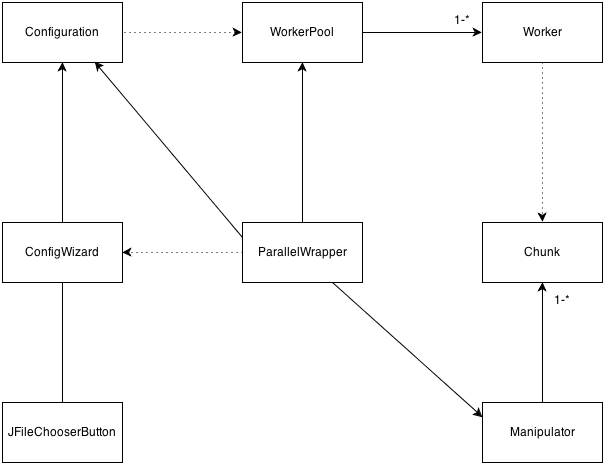
\includegraphics{figures/uml.png}}}
\caption{UML for the embarrassingly parallel framework}
\label{fig:uml}
\end{figure}
The KaKs Calculator is not the only program to use the framework; there are
various potential programs that the framework could support. The only 
requirements for the this program are that it process the input in an 
embarrassingly parallel manner and that the input comes from a file and the 
processed results are also writen to a file. The framework needs to support 
various kinds of input files and be able to chunk up the work accordingly. The 
Ka/Ks Calculator's input consists of a header and then two protein sequence 
lines followed by a blank line. The framework uses that blank line to know when 
one chunk of work has ended and another has begun. The user can input a regular 
expression to define what lines of input make up what chunks. This occurs in 
the ChunkManager class. 

The other purpose of the ChunkManager class is to combine the resulting chunks 
back together when the worker threads have finished. Once the work has been
done, all of the separate results are spread across several files. The
ChunkManager's second job is to retrieve those results and construct a real
output file. The real output file must look the same as the output file would
look if the program were run serially; the output must come in the same order as
the inputs in the input file and headers may need to be deleted from the
separate files and added to the combined file.

As more features are added to the framework and as more programs start to use 
the framework, there are more choices for the end-user to make with regards to 
how they want their program to execute. The number of threads to use, various 
flags for the executable and the statstics output are just a few choice the 
user can make. A start-up wizard is displayed at runtime to systematically allow
the end-user to choose the settings for the run. The ConfigWizard class brings 
the user through this process and creates an instance of Configuration when it 
is completed to save the user's settings.

Lastly, the worker threads will keep records during execution. The threads 
records their uptime and the number of pieces of work they execute. The runtime 
for each piece of work is also recorded. This information will be used by us to
evaluate the effectiveness of our approach, but can also provide useful
information the can help a user tine a particular application on a particular
type of input data. The statistics for each thread can be found in the Worker 
subclass and the individual Chunk classes will store their own statstics about 
runtime and size.

\section{Results}

To observe how the framework changes the runtime of sequential programs when
using varying numbers of threads, I designed a simple experiment. The Ka/Ks 
Calculator was run through the framework with ten different samples, each 
containing sixteen units of work. Each sample was run by the framework at five 
different level of numbers of worker threads, starting at 1 and increasing by 
powers of two until the 100\% CPU usage (16 processors). These tests were run
with minimal other activity on the server.

\begin{figure}
{\resizebox{5.2in}{!}{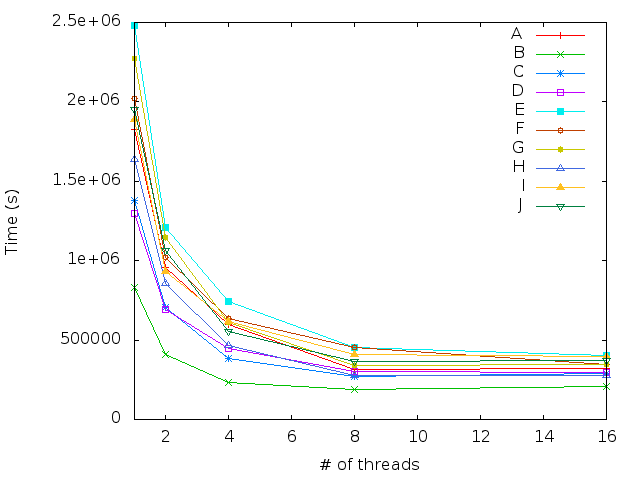
\includegraphics{experiment/out.png}}}
\caption{Runtimes for the Ka/Ks Calculator though the framework}
\label{fig:graph}
\end{figure}

\section{Conclusion}

As the numbers of threads increased, the time it took descreased exponentially. 
In a few cases, there was an increase in time when attempting to max out the CPU 
usage. This occured because the framework had to wait until for the CPU to be 
finished with its previous work before it was allowed to start work on what the 
framework wanted it to do. In the cases when the framework executed faster while
the CPU was maxed out, it was only faster a minute at the most. With such a
small time gain with the CPU at 50\% versus the CPU at 100\%, running the
framework at 50\% CPU is more efficient when the number of threads is on the
same order as the number of units of work.

There are several next steps in the pipeline. In addition to using the
statistics to try to boost speed, adding savable configurations is at the top of
the list. This will allow users to use the same configuration without having to
go through the wizard if they need to redo a run. More extensive unit testing
will be implemented. The ability to chunk multiple pieces of work may be
implemented in order to avoid potential start up costs in the executable. 
Finally, other pleasing parallel problems will be executed by the wrapper so 
that more potential features will be discovered. 

Using Java was a good choice for implementation ease and future implementation
extension by others, but it may not produce the fastest results. Languages
like Hadoop, Clojure or other multithread oriented language may have been better
due to their parallel nature. In addition to a single machine working to process
the data quickly, we can also look to the cloud for help by using a networked 
solution like MPI or a cloud solution like Amazon instances. This would
potentially allow for an even greater time decrease because the number of
machines that could help is most likely larger than the number of processors on
one machine.

\begin{thebibliography}{1}
\bibitem{history}
Moler, Cleve. ``\emph{Matrix Computation on Distributed Memory Multiprocessors."
}, Hypercube Multiprocessors, 1986: Proceedings of the First Conference on
Hypercube Multiprocessors, Knoxville, Tennessee, August 24-27, 1985. By Michael
T. Heath. Philadelphia: SIAM, 1986. N. pag. Print.
\bibitem{kaks}
Zhang Z, Li J, Zhao XQ, Wang J, Wong GK, Yu J., \emph{KaKs Calculator: 
calculating Ka and Ks through model selection and model averaging},
Genomics Proteomics Bioinformatics, November 2006.
\bibitem{cluster}
Rua, Xu, Wunsch, Donald II, \emph{Survey of Clustering Algorithms},
IEEE Transactions on Neural Networks VOL. 16, NO. 3, MAY 2005
\end{thebibliography}

\end{document}
